%!TEX root = main.tex

\section{Results}
\label{sec:results}

% \begin{figure*}
% 	\label{fig:}
% 	\caption{.}
% 	\includegraphics[width=\textwidth,height=7cm]{figures/}
% \end{figure*}

In this section, we describe some of our observations from the experiments conducted in the previous sections.




\begin{figure*}
	\label{fig:daily_earnings}
	\caption{Daily earnings.}
	%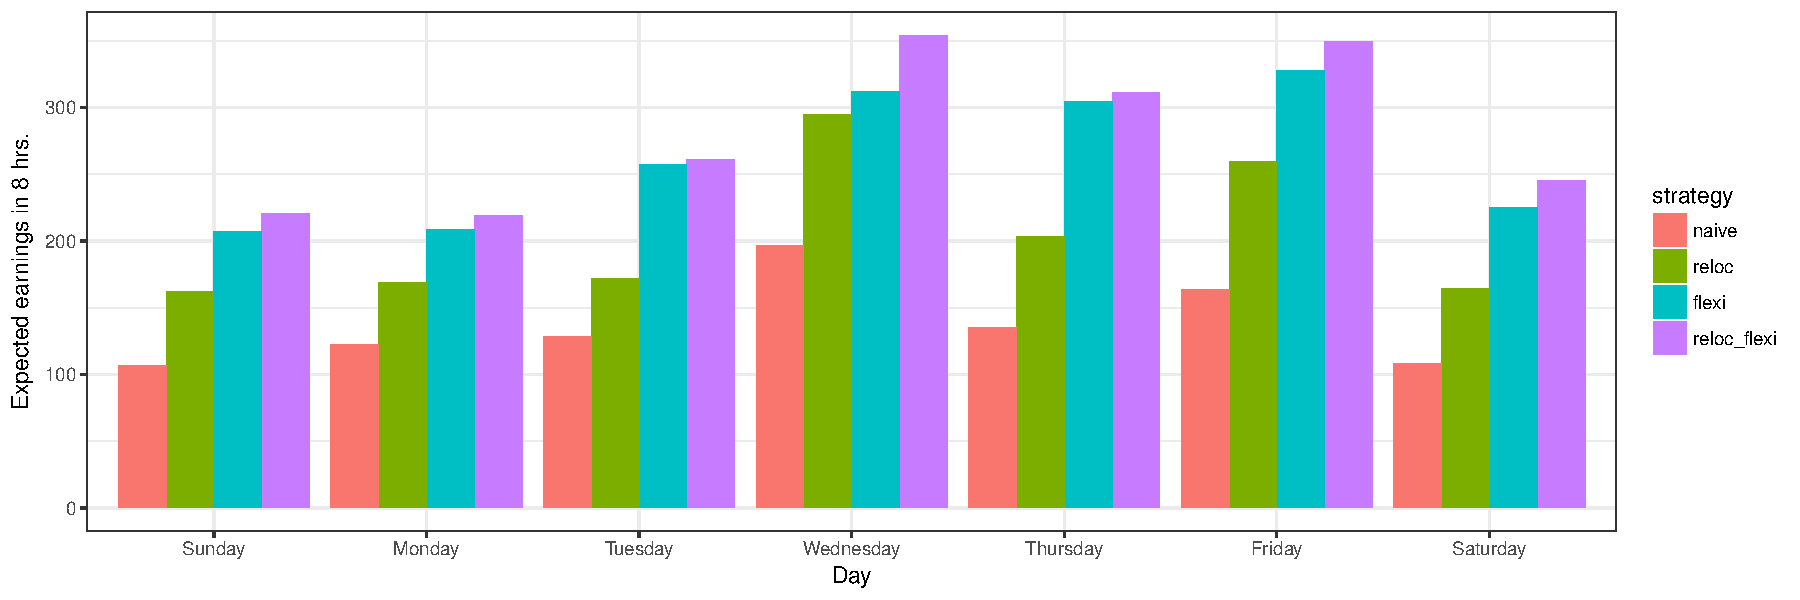
\includegraphics[width=8cm,height=4cm]{figures/daily_earnings.pdf}
	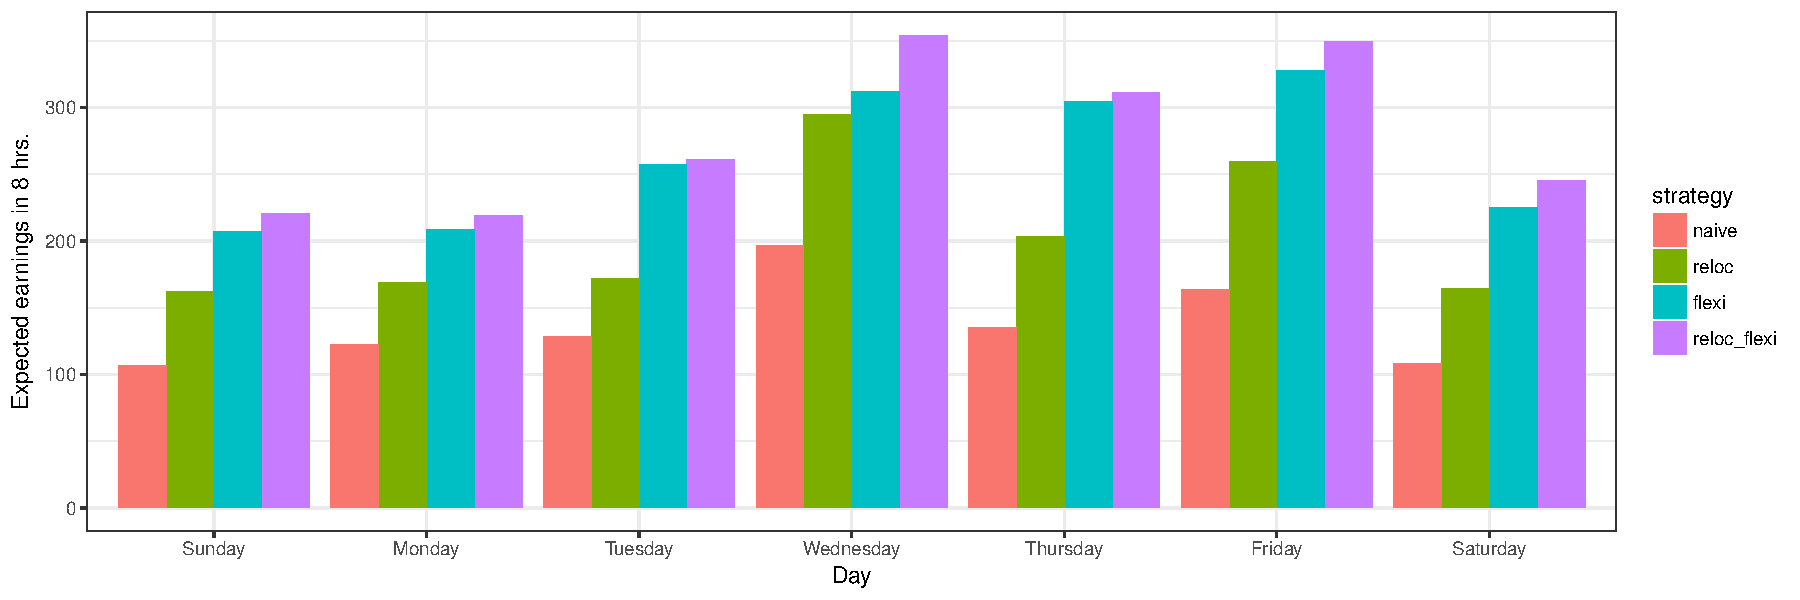
\includegraphics[scale=0.4]{figures/daily_earnings.pdf}
\end{figure*}

\begin{figure}
	\label{fig:earnings_heatmap}
	\caption{Earnings across NYC zones with \textit{naive} and \textit{reloc} strategy.}
	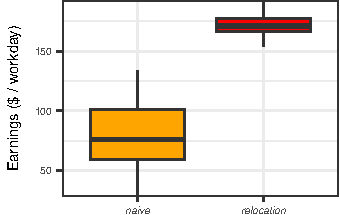
\includegraphics[width=0.7\textwidth,height=0.3\textwidth]{figures/earnings_heatmap.pdf}
\end{figure}

\begin{figure*}
	\label{fig:flexi_schedules}
	\caption{Percentage of active drivers across day using \textit{flexi} strategy.}
	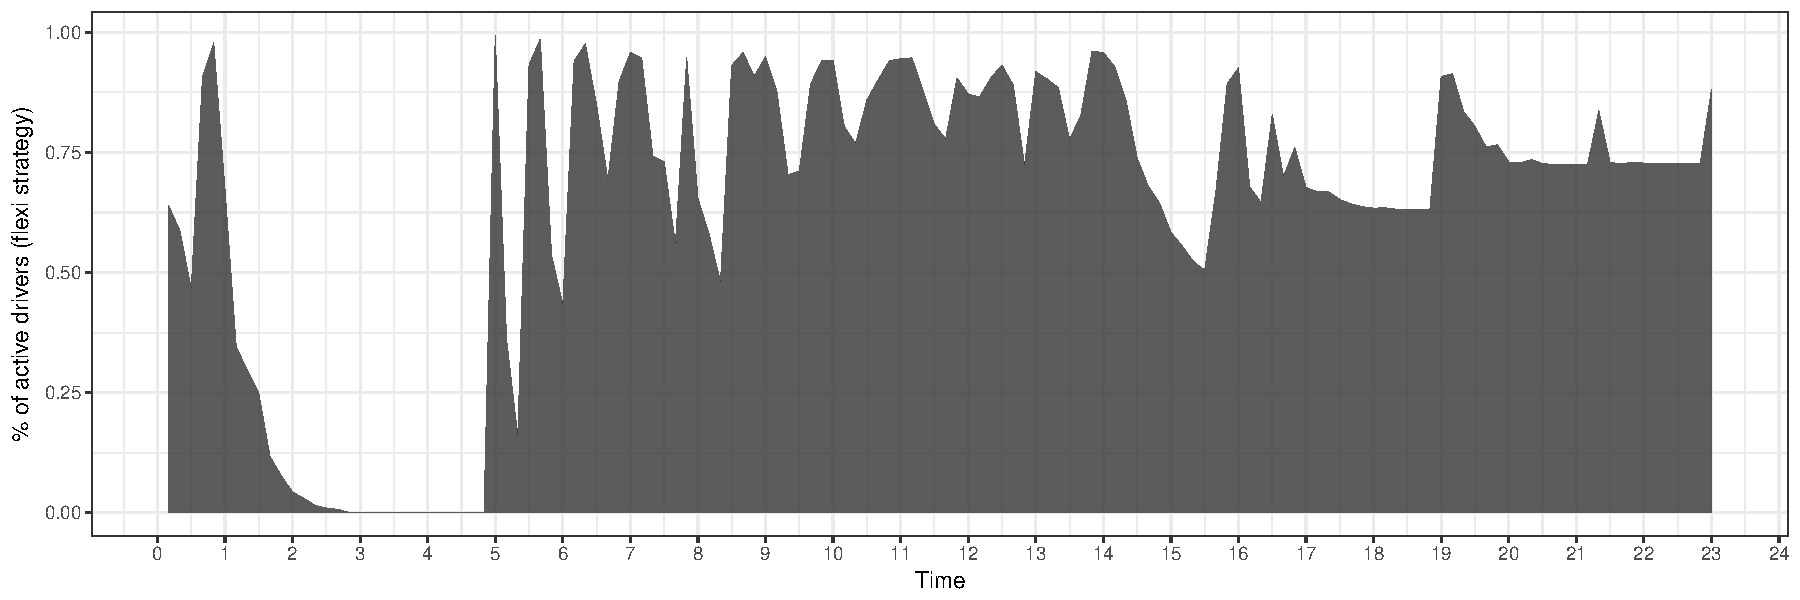
\includegraphics[width=\textwidth,height=7cm]{figures/flexi_schedules.pdf}
\end{figure*}

\begin{figure*}
	\label{fig:reloc_flexi_schedules}
	\caption{Percentage of active drivers across day using \textit{reloc\_flexi} strategy.}
	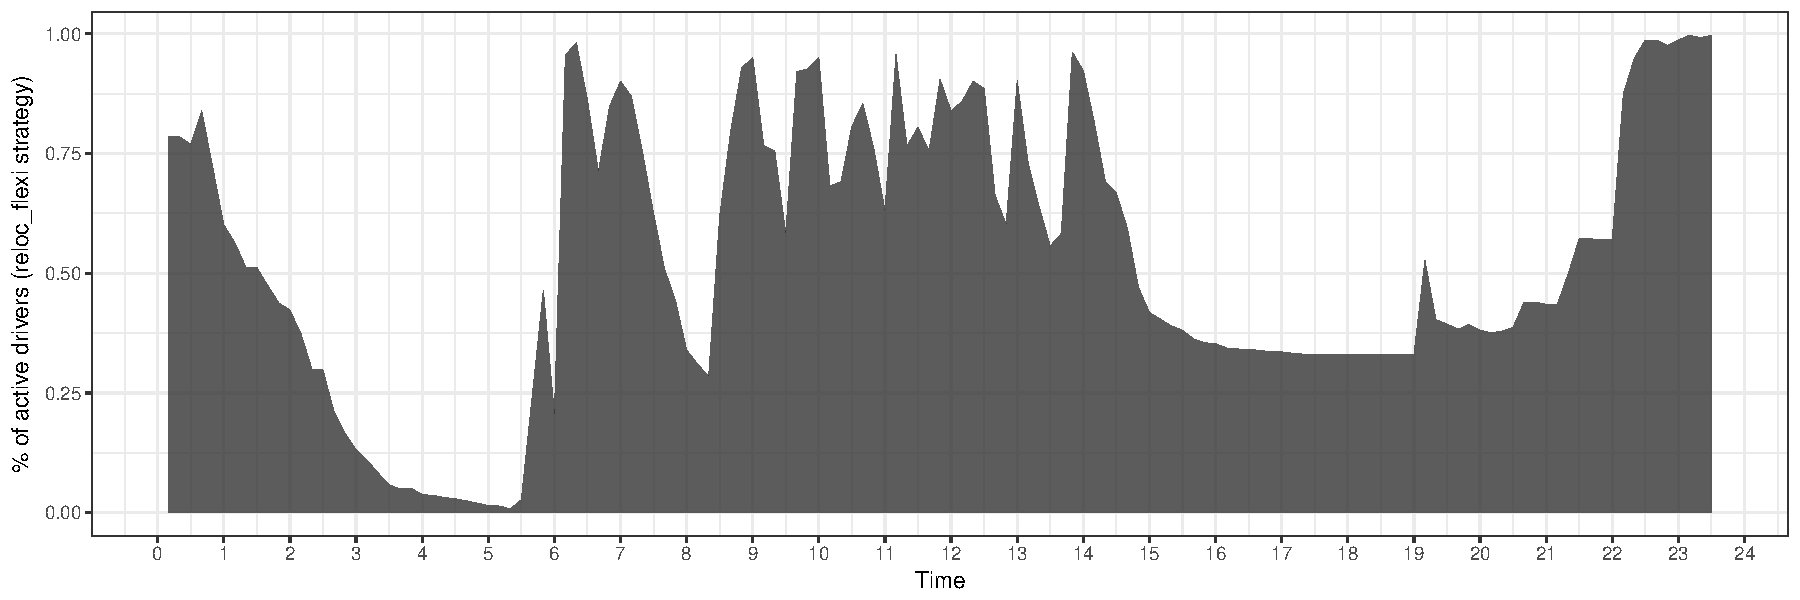
\includegraphics[width=\textwidth,height=7cm]{figures/reloc_flexi_schedules.pdf}
\end{figure*}

\begin{figure*}
	\label{fig:uncertainty_evolution}
	\caption{Uncertainty evolution.}
	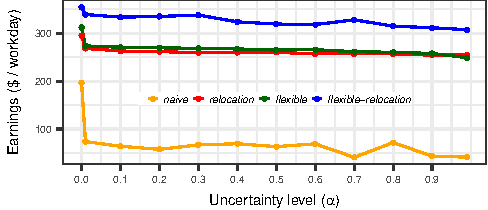
\includegraphics[width=\textwidth,height=7cm]{figures/uncertainty_evolution.pdf}
\end{figure*}

\begin{figure}
	\label{fig:simulated_earnings}
	\caption{Simulated earnings for drivers across different strategies.}
	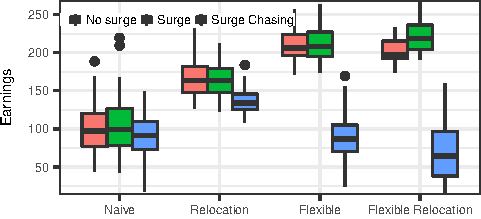
\includegraphics[width=0.5\textwidth,height=0.4\textwidth]{figures/simulated_earnings.pdf}
\end{figure}

\begin{figure*}
	\label{fig:reloc_end_zones}
	\caption{Popular relocation destinations for \textit{reloc} strategy.}
	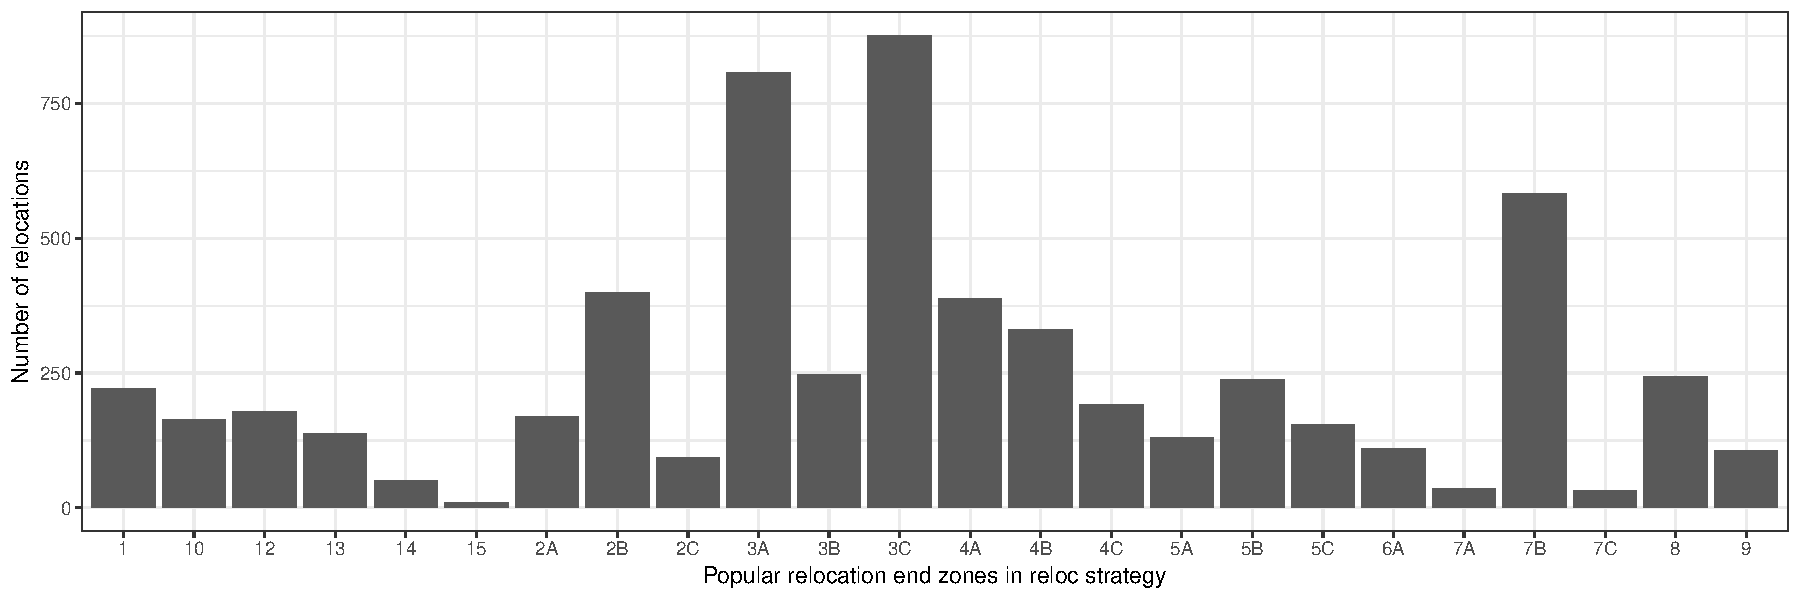
\includegraphics[width=\textwidth,height=7cm]{figures/reloc_end_zones.pdf}
\end{figure*}

\begin{figure*}
	\label{fig:reloc_flexi_end_zones}
	\caption{Popular relocation destinations for \textit{reloc\_flexi} strategy.}
	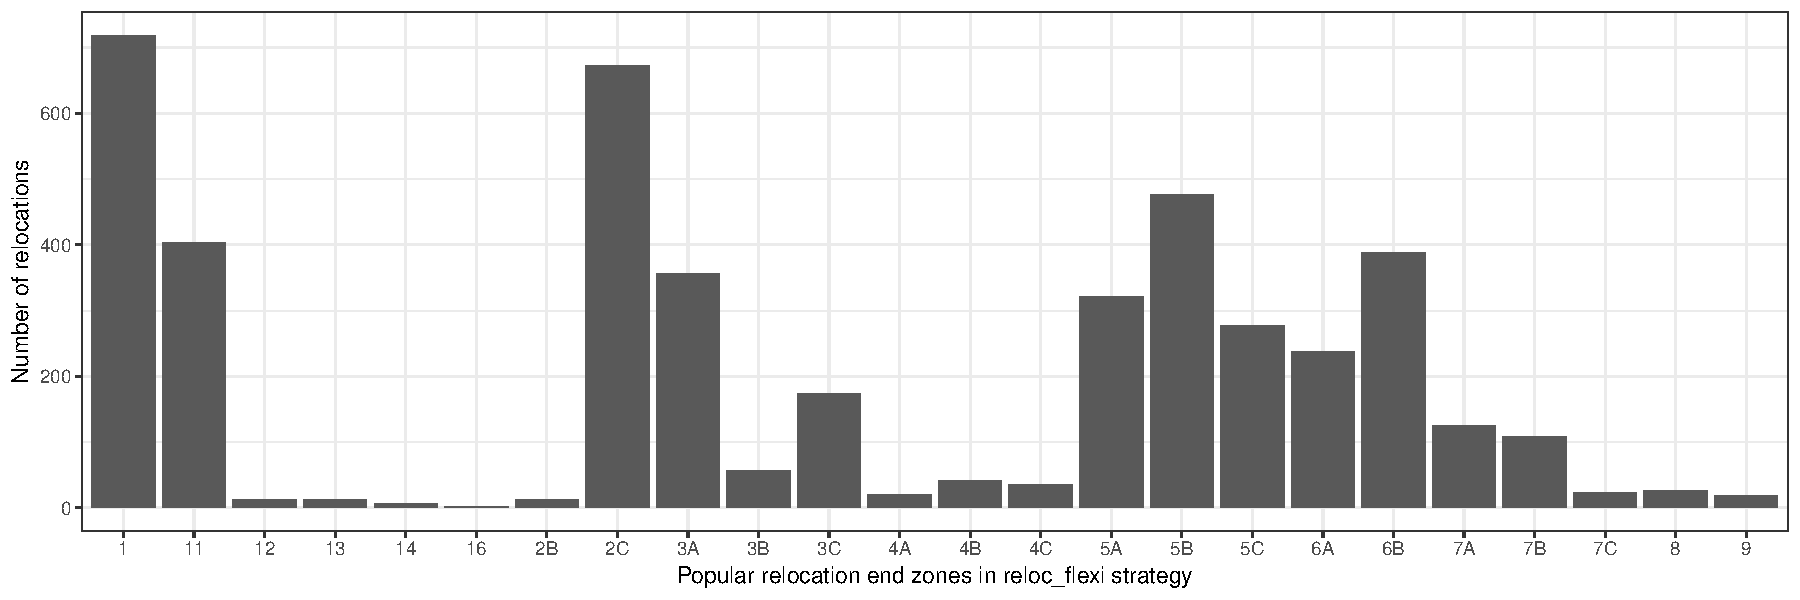
\includegraphics[width=\textwidth,height=7cm]{figures/reloc_flexi_end_zones.pdf}
\end{figure*}
